\documentclass[tikz,border=5mm,12pt]{standalone}
\usepackage[fontsize=16pt]{fontsize}
\usetikzlibrary{arrows.meta}

\newcommand\vsep{10mm}
\newcommand\textwidthfirst{65mm}
\newcommand\textwidthsecond{100mm}

\begin{document}
  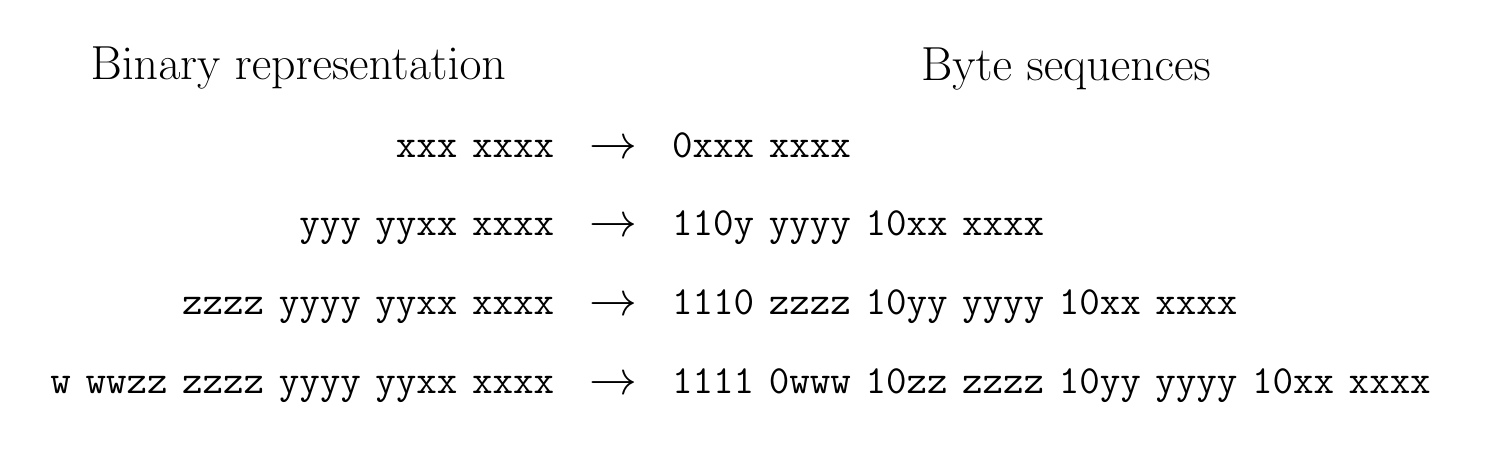
\begin{tikzpicture}
    \node[text width=\textwidthfirst,align=center] at (0,0) {Binary representation\strut};
    \node[text width=\textwidthfirst,align=right] at (0,-1*\vsep) {\small\texttt{xxx xxxx}\strut};
    \node[text width=\textwidthfirst,align=right] at (0,-2*\vsep) {\small\texttt{yyy yyxx xxxx}\strut};
    \node[text width=\textwidthfirst,align=right] at (0,-3*\vsep) {\small\texttt{zzzz yyyy yyxx xxxx}\strut};
    \node[text width=\textwidthfirst,align=right] at (0,-4*\vsep) {\small\texttt{w wwzz zzzz yyyy yyxx xxxx}\strut};

    \node at (40mm,-1*\vsep) {$\rightarrow$\strut};
    \node at (40mm,-2*\vsep) {$\rightarrow$\strut};
    \node at (40mm,-3*\vsep) {$\rightarrow$\strut};
    \node at (40mm,-4*\vsep) {$\rightarrow$\strut};

    \node[text width=\textwidthsecond,align=center] at (97.5mm,0) {Byte sequences};
    \node[text width=\textwidthsecond,align=left] at (97.5mm,-1*\vsep) {\small\texttt{0xxx xxxx}\strut};
    \node[text width=\textwidthsecond,align=left] at (97.5mm,-2*\vsep) {\small\texttt{110y yyyy 10xx xxxx}\strut};
    \node[text width=\textwidthsecond,align=left] at (97.5mm,-3*\vsep) {\small\texttt{1110 zzzz 10yy yyyy 10xx xxxx}\strut};
    \node[text width=\textwidthsecond,align=left] at (97.5mm,-4*\vsep) {\small\texttt{1111 0www 10zz zzzz 10yy yyyy 10xx xxxx}\strut};

  \end{tikzpicture}
\end{document}
